\subsection{Arquitectura de clases Ip}

Al principio las direcciones se interpretaban como 8 bits para la direccion de red y 24 para la dirección del host: \textcolor{red}{154}.\textcolor{blue}{200}.\textcolor{blue}{31}.\textcolor{blue}{1}

Luego se introduce el \textbf{Classful  Addresing} para dividir el espacion de direcciones en clases:

\begin{itemize}
    \item Clase A: \textcolor{red}{10}.\textcolor{blue}{20}.\textcolor{blue}{0}.\textcolor{blue}{7}
    \item Clase B: \textcolor{red}{154}.\textcolor{red}{13}.\textcolor{blue}{22}.\textcolor{blue}{3}
    \item Clase C: \textcolor{red}{200}.\textcolor{red}{4}.\textcolor{red}{67}.\textcolor{blue}{3}
    \item Clase D: Multicast
    \item Clase E: Experimental
\end{itemize}

Posteriormente se introduce \textbf{e Classless Inter-Domain Routing (CIDR)} que implica máscaras de subred de longitud variable: 200.4.67.3 \textcolor{yellow}{/23}

\subsection{Subnets}

Una subnet es una subdivision lógica de una red, permitiendo agrupar direcciones en un rango. Se describen por ejemplo: 192.168.1.0/24.
La máscara permite reducir la lógica que tienen que manejar los routers, permitiendo separar el tráfico en subredes optimizando el uso de la red. A su vez reduciendo la congestion de red, aumentando la seguridad y facilitando la administracion de la red.

\subsection{Ejercicios}

En los ejercicios de subnetting, dada una subred se busca maximizar la cantidad de direcciones ocupada ya que cada direccion inactiva desperciada es plata tirada.

\subsubsection{Metodologia}
Todas las subredes tienen una direccion de red y una direccion de broadcast. No se puede asignar la direccion de red o la de broadcast a un host. Todos los dispositivos conectados a la red tienen una dirección IP (los routers también).

$$ \mathrm{\# de hosts} = 2^{32-\mathrm{mascara}}-2 $$ 

El último 2 restando se debe a que las direcciones de red y broadcast no se pueden usar

\subsubsection{Ejercicio 1}

\begin{figure}[H]
\centering
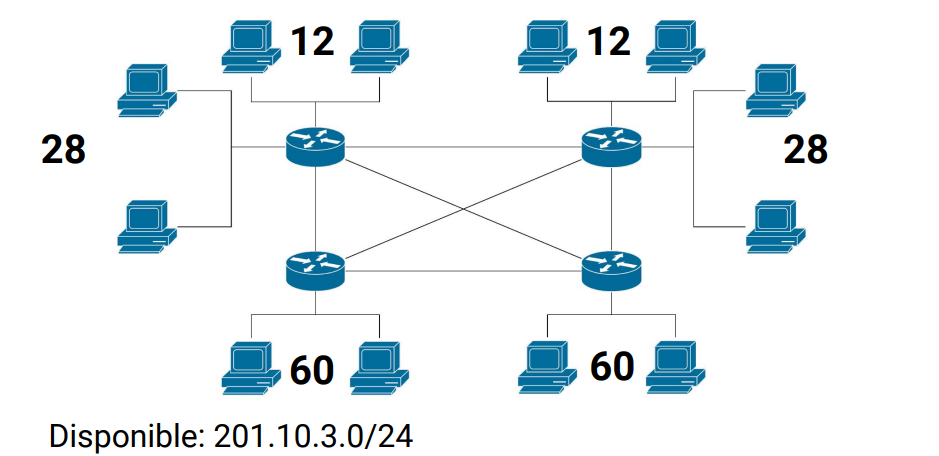
\includegraphics[width=\textwidth]{imagenes/enunciado1subnetting.png}
\end{figure}

A priori se pueden identificar 6 subredes (cada una con la cantidad de hosts), 4 routers y 6 enlaces entre routers. Hay que tener en cuenta que \textcolor{red}{los enlaces punto a punto entre routers necesitan tener su propia subred}. De esta manera, quedan 12 subredes, 4 routers y 6 enlaces entre routers. Ademas \textcolor{red}{201}.\textcolor{red}{10}.\textcolor{red}{3}.\textcolor{blue}{0}. Entonces se tienen 8 bits para las direcciones de host, es decir 256 direcciones

\begin{figure}[H]
\centering
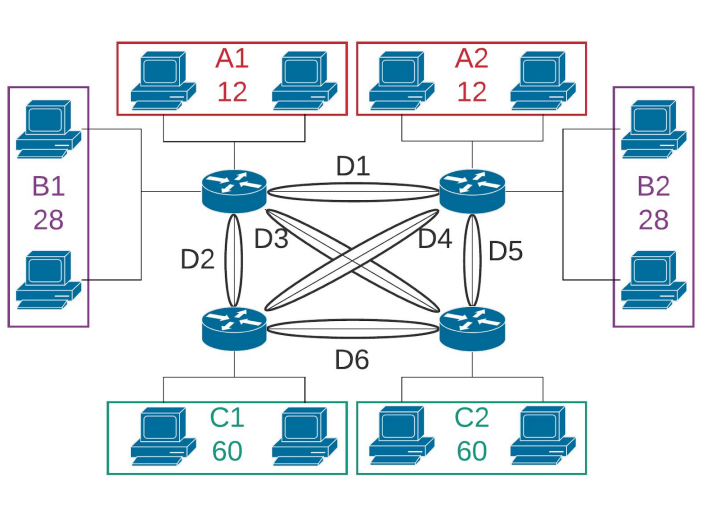
\includegraphics[width=\textwidth]{imagenes/subnetting12.png}
\end{figure}

Para delimitar las subredes:

\begin{itemize}
    \item Ver cuantos hosts tiene cada uno (sin olvidar los routers)
    \item Averiguar el espacio de direcciones a subdividir
    \item asignar la minima cantidad de IP a cada subred
\end{itemize}

Las redes con más hosts son \textbf{C1} y \textbf{C2} con 60 hosts más un router cada una. Como las 256 direcciones disponibles son mayores a las 61 que precisa la red, se divide en 2 la red. Se tienen 2 redes /25 con 128 direcciones cada una.

\begin{figure}[H]
\centering
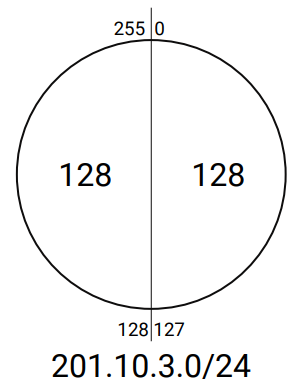
\includegraphics[width=0.3\textwidth]{imagenes/subnetting13.png}
\end{figure}


\begin{figure}[H]
\centering
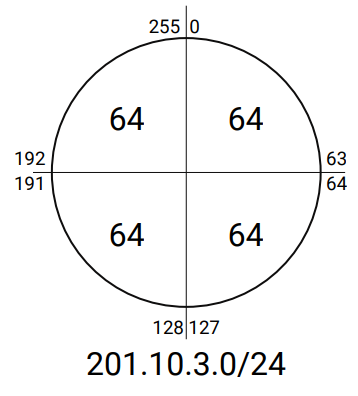
\includegraphics[width=0.3\textwidth]{imagenes/subnetting14.png}
\end{figure}


Sin embargo sigue siendo muy mayor 128 a 61, entonces se divide la red nuevamente. Se tienen 4 redes /26 con 64 direcciones cada una. Si dividiera nuevamente, quedarian redes con 32 direcciones, insuficientes para C1 y C2. Entonces asigno a C1 y a C2 a cada espacio de 64 direcciones

\begin{figure}[H]
\centering
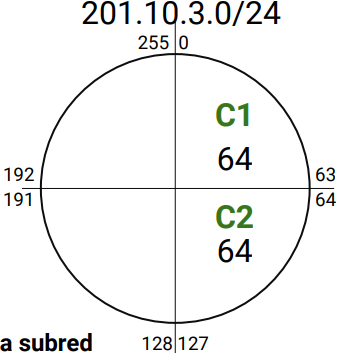
\includegraphics[width=0.3\textwidth]{imagenes/subnetting15.png}
\end{figure}

De esta manera, las direcciones de las subredes quedarian asignadas de la siguiente manera:

\begin{center}
    \begin{tabular}{c|c}
    Subred & Dirección de la subred \\
    \hline
    \hline
    C1     & 201.10.3.0 / 26 \\
    C2     & 201.10.3.64 / 26
    \end{tabular}
\end{center}


Las redes siguientes en tamaño son B1 y B2 con 28 hosts cada una. Quedan 2 redes de 64, puede dividirse una y quedan de 32 para asignar.


\begin{center}
    \begin{tabular}{c|c}
    Subred & Dirección de la subred \\
    \hline
    \hline
    C1     & 201.10.3.0 / 26 \\
    C2     & 201.10.3.64 / 26 \\
    B1     201.10.3.128 / 27 \\
    B2     & 201.10.3.160 / 27
    \end{tabular}
\end{center}


\begin{figure}[H]
\centering
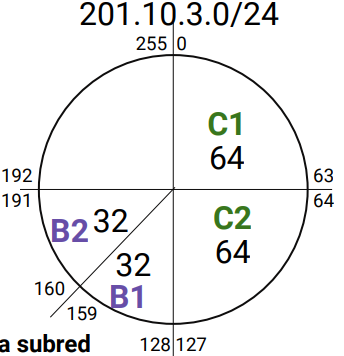
\includegraphics[width=0.3\textwidth]{imagenes/subnetting16.png}
\end{figure}

Se procede de igual manera con las redes que siguen en cantidad de hosts


\begin{center}
    \begin{tabular}{c|c}
    Subred & Dirección de la subred \\
    \hline
    \hline
    C1     & 201.10.3.0 / 26 \\
    \hline
    C2     & 201.10.3.64 / 26 \\
    \hline
    B1     & 201.10.3.128 / 27 \\
    \hline
    B2     & 201.10.3.160 / 27 \\
    \hline
    A1     & 201.10.3.192 / 28 \\
    \hline
    A2     & 201.10.3.208 / 28 \\
    \hline
    D1     & 201.10.3.224 / 30\\
    \hline
    D2     & 201.10.3.228 / 30 \\
    \hline
    D3     & 201.10.3.232 / 30 \\
    \hline
    D4     & 201.10.3.236 / 30\\
    \hline
    D5     & 201.10.3.240 / 30 \\
    \hline
    D6     & 201.10.3.244 / 30 \\
    \end{tabular}
\end{center}


\begin{figure}[H]
\centering
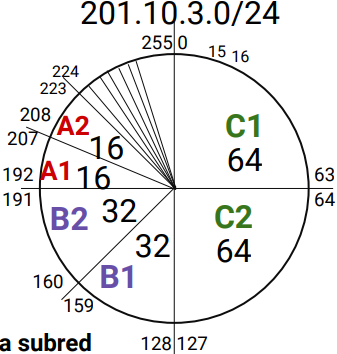
\includegraphics[width=0.3\textwidth]{imagenes/subnetting17.png}
\end{figure}


\subsubsection{Ejercicio 2}

Dada la siguiente configuración de hosts y routers, y el espacio 192.168.0.0/23, se pide separar en subredes minimizando la cantidad de IPs sin usar. Ante igualdad de condiciones para ubicar varias subredes:
\begin{itemize}
    \item Asignar bloques utilizando los prefijos en orden de numeración ascendente (Ej: si tenemos la opcion de usar 117.0.1.0/24 o 117.0.0.0/24, debemos utilizar primero el espacio de direcciones 117.0.0.0/24).
    \item  Asignar bloques de direcciones priorizando las redes con mayor cantidad de hosts (Ej: si se deben asignar dos bloques de 64 direcciones IP para dos subredes distintas Sx y Sy , donde x e y representan la cantidad de hosts de cada subred y con 32 < x < y < 64, Sy debe asignarse en un espacio de direcciones de menor numeración).
    \item Si dos subredes necesitan la misma cantidad de IPs, ubicar primero la subred cuya letra viene primero en el abecedario (Ej: si las redes P y J tienen necesitan un bloque de 32 IPs, ubicar primero la J y luego la P).
\end{itemize}
Este criterio arbitrario define una única resolución posible de la configuración. Cualquier otra solución será considerada incorrecta.

\begin{figure}[H]
\centering
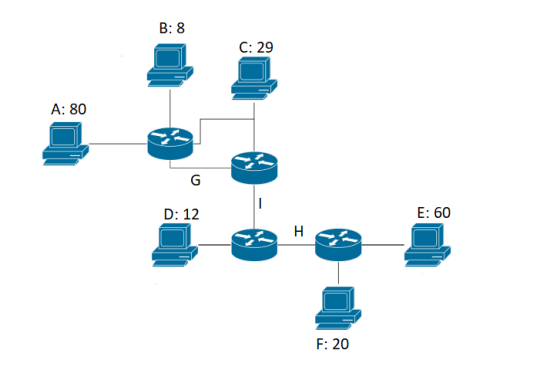
\includegraphics[width=\textwidth]{imagenes/subnetting2.png}
\end{figure}


El espacio es 192.168.0.0/23 entonces para los hosts se tienen 9 bits, es decir un rango de 512 direcciones: de 0 (0.0) a 511 (0.255).

\begin{center}
     \begin{tabular}{c|c|c|c}
          0-7 & 8-15 & 16-23 & 24-31 \\
          \hline
          192 & 168 & 0000000 \textbf{0} & \textbf{00000000}
     \end{tabular}
\end{center}

\begin{figure}[H]
\centering
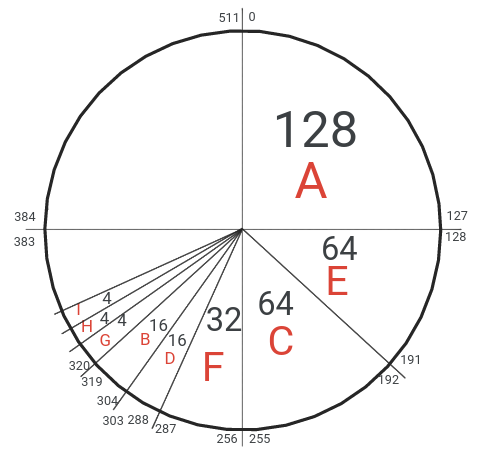
\includegraphics[width=0.5\textwidth]{imagenes/subnettingTorta.png}
\end{figure}


La subnet con más hosts es la A con 80. Hay que tener en cuenta que tiene un router, una direccion de red y una de broadcast, necesitando en total 83 direcciones. Puedo dividir hasta una sección de 128 direcciones. Entonces el espacio para A será  192.168.0.0/25 (25 porque arrancaba con una mascara de 23 y se dividió 2 veces el espacio original).\\
El que sigue en cantidad de hosts es E con 60, ademas de los 2 routers y las 2 direcciones a reservar da un total de 64. Puede subdividirse una sección de 128 direcciones a una sección de 64 direcciones. La máscara será de 26 y el espacio será desde 192.168.0.128.\\
En tamaño sigue la subnet C con 29, suado a 2 routers y las 2 direcciones da 33. Se debe usar una seccion de 64. La máscara quedará de 26 y el espacio irá desde 192.168.0.192.\\
Sigue F con 20 hosts, un router y dos direcciones reservadas por un total de 23 direcciones, entonces la máscara queda de 27 y el espacio irá desde 192.168.1.0. Se usa un bloque de 32.\\
Sigue D con 12 hosts, 1 router y dos direcciones por un total de 15, se puede dividir una seccion de 32 a una de 16. La máscara quedará entonces de 28 y el espacio irá desde 192.168.1.32.\\
Sigue B con 8, 1 router y 2 direcciones por un total de 11. Entonces se usa un bloque de 16. La máscara queda entonces de 28 y el espacio irá desde 192.168.1.48.\\
Cada router tiene 2 routers y 2 direcciones, por lo que se asignan bloques de 4, con máscaras de 30\\


\begin{center}
    \begin{tabular}{c|c|c|c|c}
        Subnet & \#Host & \#Router & Block & Prefix/Mask \\
        \hline
        \hline
        A & 80 & 1 & 128 & 192.168.0.0/25\\
        \hline
        B &  8 & 1 & 16 & 192.168.1.48/28\\
        \hline
        C &  29 & 2 & 64 &  192.168.0.192/26\\
        \hline
        D &  12 & 1 & 16 & 192.168.1.32/28 \\
        \hline
        E &  60 & 1 & 64 & 192.168.0.128/26 \\
        \hline
        F &  20 & 1 & 32 & 192.168.1.0/27 \\
        \hline
        G &  0 & 2 & 4 & 192.168.1.64/30  \\
        \hline
        H &  0 & 2 & 4 & 192.168.1.68/30  \\
        \hline
        I &  0 & 2 & 4 & 192.168.1.72/30 \\
        
    \end{tabular}
\end{center}